\documentclass[11pt,a4paper]{article}
\usepackage{od,wrapfig,array}
\usepackage[utf8]{inputenc}
\usepackage[main=german,russian]{babel}

\pagestyle{headings}
\title{TRIZ Summit Cup – 2020/2021}
\setcounter{tocdepth}{2} 
\author{(Nicht autorisierte) Übersetzung ins Deutsche von Hans-Gert Gr\"abe,
  Leipzig} 
\date{November 23, 2020}

\begin{document}
\maketitle
\tableofcontents
\enlargethispage{12em}
\clearpage
\section{Kategorie 8-10 Jahre}

\subsection{Nomination „Erfinden“}

\subsubsection*{Aufgabe 1. Der Marsrover.}
Eine fantastische Geschichte beschreibt eine Expedition zum Mars.  Das
Raumschiff ging in einem Tal mit einer sehr unebenen Oberfläche herunter:
überall Hügel, Gruben, Steine. Die Astronauten rüsteten schnell ein
Geländefahrzeug aus -- ein Radfahrzeug mit großen aufblasbaren Reifen. Doch am
ersten Steilhang kippte der Geländewagen zur Seite. Und dann... Nein, leider
gab es in der Geschichte keinen Erfinder. Was denkst du: Was hätte er
vorgeschlagen? Beachte, dass die Astronauten nicht die Möglichkeit hatten, das
Geländefahrzeug umzubauen.  (Eine Aufgabe aus dem Buch von G.S. Altschuller
„Und dann kam der Erfinder“ -- \foreignlanguage{russian}{И тут появился
  изобретатель}. Eine Übersetzung des relevanten Ausschnitts aus dem Buch ist
diesen Materialien beigefügt).

Analysiere die Kontrolllösung (im Buch angegeben): Finde das Konfliktpaar,
formuliere den Widerspruch, das IER, beschreibe, mit welchem Vorgehensmuster
der Widerspruch gelöst werden kann. Schlage andere Lösungen vor.

\subsubsection*{Aufgabe 2. Der Fahrer des Mondfahrzeugs.}
Du liebst Rennwagenmodelle mit Fernsteuerung fahren oder das Fahren auf einer
schwierigen Strecke im Fahrsimulator?  Jetzt stelle dir vor, du bist der
Fahrer eines Mondfahrzeugs, eines echten Transportmittels, das in der Lage
sind, auf dem Mond herumzufahren. Im November 1970 hat das unbemannte
Raumschiff „Luna 17“ den \emph{Lunochod} als erstes solches Fahrzeug auf dem
Erdtrabanten abgesetzt, um die Oberfläche des Mondes direkt zu untersuchen.
Die Steuerung des Lunochod übernahm eine Gruppe von 11 Personen in mehreren
Schichten, die aus folgenden Personen bestand: dem Kommandanten, dem Fahrer,
dem Antennenausrichter, dem Steuermann und dem Bordingenieur. Während der
Ausbildung der Fahrer auf dem Lunodrom entstand ein Problem -- der Lunochod
wurde ferngesteuert, d.h. der Fahrer sieht den Lunochod auf einem Bildschirm,
und die Kommandos, die er sendet, werden erst nach 3-5 Sekunden ausgeführt
(Laufzeit des Signals zum Mond und zurück sowie für die Signalverarbeitung) --
dies ist sehr ungewöhnlich für den Fahrer und erfordert ein langes Training.
Hier ist eine Episode des Trainings: „Die Motoren sind eingeschaltet. Der
Lunochod rückt vorwärts und bleibt gleich wieder stehen -- der Fahrer befahl
ihm zu stoppen, und die Maschine folgte dem Befehl.  Aber derMensch konnte
nicht erklären, warum er das Experiment abbrach -- ihm schien es, dass der
Lunochod sich seitwärts bewegte.  Die Telesteuerung war nicht so einfach.  Es
fehlte der Raum, an den die Augen so gewöhnt sind. Nach 15 Minuten stand der
Fahrer von seinem Sessel auf. Und obwohl der Raum ziemlich kühl war, konnte
man sein Hemd auswringen -- die Arbeit vor dem Bildschirm erforderte eine hohe
Anspannung. Nach mehreren Stunden am Bildschirm hatte sich der Fahrer an die
Situation „gewöhnt“, und der Lunochod folgte gehorsam, aber am nächsten Tag
fing alles wieder von vorne an -- die erlernten Fähigkeiten ware wieder
verloren gegangen“.  Die Situation ist klar: Die Fähigkeiten, den Lunochod
über Bildschirm zu steuern, sollten möglichst lange erhalten bleiben, aber es
ist unmöglich, die ganze Zeit auf der Trainingsstation zu verbringen. Was
schlägst du dem Lunochod-Fahrer vor, wie kann er in seinem normalen Leben
seine Fernsteuerfähigkeiten weiter verbessern?  Formuliere Widersprüche, das
IER, berücksichtige die verfügbaren Ressourcen.

\subsection{Nomination „Fantasieren“}

\subsubsection*{Aufgabe 1.}
In Arthur C. Clarkes Roman \emph{Rendevouz mit Rama} wird ein außerirdisches
Raumschiff beschrieben, das bis zu 50 Kilometer groß ist. Verwende die
„Zoom“-Technik und beschreibe das größte Raumschiff, das du dir vorstellen
kannst.

\subsubsection*{Aufgabe 2.}

Im Science-Fiction-Roman \emph{Das dritte Jahrtausend} von Heinrich Altov (dem
Schriftsteller-Pseudonym von G.S. Altschuller) wird beschrieben, wie Menschen
den Planeten Jupiter in Gas und Staub zermalmt haben (Anwendung des
TRIZ-Prinzips der „Zerlegung“). Es entstand eine riesige Gaswolke um die
Sonne, die so dicht ist wie die Atmosphäre der Erde. Man kann darin in
Düsen-Jets von Planet zu Planet fliegen und sogar mit Ballons. In der
interplanetaren Gaswolke entstehen Wolkengebilde und Wolken, es blitzt. Denke
dir eine Geschichte über die Abenteuer von Kindern aus, die mit einem Ballon
zum Mars reisen.

\subsection{Nomination „TRIZ-Werkzeuge“}

\subsubsection*{Aufgabe 1.}
Die Erkundung des Kosmos bringt aufregende Abenteuer, außergewöhnliche
Entdeckungen und Freude, das Unbekannte zu erkennen, mit sich. Diese
Forschungen haben auch rein praktische Anwendungen. Du weißt sicher, dass
Teflonbeschichtung, drahtlose Elektrowerkzeuge, Geolokalisierungsdienste und
viele andere Erfindungen, die unser Leben bequemer und sicherer machen, in der
Raumfahrtindustrie entstanden sind. Die Aufgaben in der Kategorie
„TRIZ-Werkzeuge“ sind mit solchen Erfindungen verbunden.

\begin{itemize}[noitemsep]
\item[1)] Lege einen Katalog „kosmischer Erfindungen“ an, die Einzug ins
  tägliche Leben gehalten haben.
\item[2)] Formuliere Widersprüche, die in diesem Erfindungen gelöst wurden. 
\item[3)] Schlage ungewöhnliche Anwendungen dieser Erfindungen für das Lösen
  noch nicht gestellter Aufgaben vor.
\end{itemize}

\subsubsection*{Aufgabe 2.}

Märchen, Mythen, Legenden sind oft der einzige Weg, um herauszufinden, wie sie
unsere fernen Vorfahren gelebt haben. Und es ist so interessant, was auf
unserer Erde vor vielen Jahrhunderten geschah, welche Geschichten erzählt
wurden, wie die Häuser aussahen, was unsere Vorfahren gedacht und geträumt
haben. Und möchtest du nicht auch, dass über deine Familie, deine Freunde,
deine Stadt Menschen nach vielen Tausend Jahren erfahren?  Denke dir ein
Märchen, Mythos, Legende, fantastische Geschichte aus, die so interessant ist,
dass sie auch noch nach Hunderten von Jahren erzählt wird.

\subsection{Nomination „Forschung“}

\subsubsection*{Aufgabe 1.}

\newcommand{\AnimalsInCosmos}{Seit den Anfängen der Erforschung des Weltraums
  wurde der Mensch von Tieren begleitet (und manchmal ersetzt). In den mehr
  als 60 Jahren Weltraumforschung sind alle möglichen Arten von Tieren sind im
  Weltraum gewesen. Die interessantesten Experimente im Orbit stehen im
  Zusammenhang mit der Kultivierung von Pflanzen. Es war nicht sofort möglich,
  Bedingungen zu schaffen, unter denen die Pflanzen nicht nur grüne Masse
  ansetzten, sondern auch blühten und Früchte trugen. Hier also das
  Forschungsthema: „Tiere und Pflanzen im Weltraum“.  Du kannst für deine
  Untersuchungen ein spezifischeres Thema wählen.
\begin{itemize}[noitemsep]
\item Katalog „Tiere im Weltraum“. Art der Tiere, Datum des Fluges ins All,
  Dauer des Aufenthalts im Weltraum, Ziele des Experiments, Ergebnisse des
  Experiments.
\item Katalog „Pflanzen im Weltraum“. Art der Pflanze, Datum des Fluges ins
  All, Dauer des Aufenthalts im Weltraum, Ziele des Experiments, Ergebnisse
  des Experiments.
\item Katalog „Geräte zur Aufrechterhaltung der Lebenstätigkeit von Tieren im
  Kosmos“.  Welche Aufgaben standen und wie wurden diese in jedem der Geräte
  gelöst?
\item Katalog „Geräte zur Aufrechterhaltung der Lebensaktivität von Pflanzen
  im Kosmos“.  Welche Aufgaben standen und wie wurden diese in jedem der
  Geräte gelöst?
\item Welche Aufgaben der Anpassung von Tieren und Pflanzen an den Aufenthalt
  im Weltraum sind immer noch ungelöst?  Schlage mögliche Lösungen vor.
\end{itemize}}

\AnimalsInCosmos

\subsection{Nomination „TRIZ-Videos“}

\newcommand{\VideoOne}{Gibt es in deiner Stadt Orte, die mit der Erforschung
  des Kosmos in Zusammenhang stehen?  Erstelle einen Bericht über einen
  Museumsbesuch, eine Ausstellung, eines Wissenschaftszentrums. Versuche,
  Raumfahrt-Experten zu ihren Kosmosforschungen zu befragen. }

\newcommand{\VideoTwo}{Illustriere mit den Mitteln Film oder Animation, wie
  erfinderische Probleme gelöst werden. Lasse dir eine Geschichte einfallen,
  in der ein Problem auftritt, versuche, im Detail zu kommentieren, worin der
  Widerspruch besteht, welche ideale Lösung erreicht werden soll und welche
  Techniken zur Lösung verwendet werden.}

\newcommand{\GeneralText}{Die Videos sollten kurz sein (2 bis 10 Minuten).
  Alle Autoren des Videos müssen angegeben werden: der Autor des Drehbuchs,
  der Operator, der Cutter, die Schauspieler, usw.  Diese Arbeit soll auf die
  Erstellung von methodischem Material für die TRIZ-Ausbildung abzielen. Auf
  der Website des TRIZ-Summit sind Videos veröffentlicht, die für den letzten
  TRIZ Summit Cup eingereicht wurden: \\
  \url{http://triz-summit.ru/ru/contest/competition/video/}\\
  \url{https://www.youtube.com/channel/UCjMNOjboWRBQA72DJvaC7ew/featured}

  An der Vorbereitung der Aufgaben des TRIZ Summit Cups 2020/2021 waren
  M.S. Rubin und N.V. Rubina beteiligt, die Nominierung „Fantasieren“ wurde
  von P.R. Amnuel' vorbereitet.}

\subsubsection*{Aufgabe 1.}\VideoOne
\subsubsection*{Aufgabe 2.}\VideoTwo

\GeneralText
\clearpage

\section{Kategorie 11-14 Jahre}

\subsection{Nomination „Erfinden“}

\subsubsection*{Vorbemerkung. Die weiche Marslandung.}

\begin{wrapfigure}{r}{.3\textwidth}\vspace*{-1em}\centering
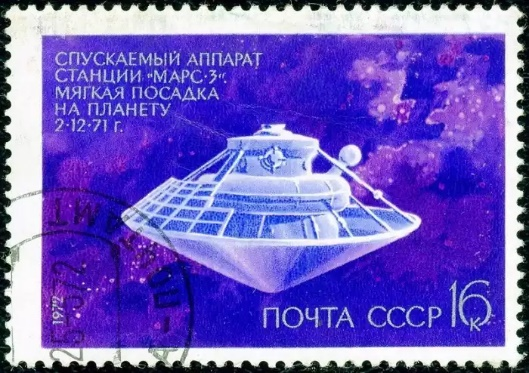
\includegraphics[width=.25\textwidth]{jEMlaM.jpg}
\end{wrapfigure}
Der Traum vieler Weltraumforscher bleibt ein Flug zum Mars. Das erste
künstliche Objekt, das die Oberfläche des Roten Planeten berührte, war der
Marsrover PROP-M\footnote{Die Abkürzung steht für die russischen Worte
  \foreignlanguage{russian}{Прибор оценки проходимости - Марс}, Gerät zur
  Beurteilung der Geländegängigkeit auf dem Mars}. Am 2. Dezember 1971
erfolgte die weiche Landung.  Versuchen wir, einen Teil des Weges zum Mars
samt Landeanflug, den Marsrover und Überlegungen seiner Konstrukteure
nachzuvollziehen. Die Landekapsel hat also die Grenzen der Marsatmosphäre
erreicht, es beginnt die aerodynamische Bremsung.  Für die weiche Landung wird
ein Fallschirmsystem verwendet.

\subsubsection*{Aufgabe 1.}
Um ein Fallschirmsystem zu starten, wird ein Auswurf-Fallschirm verwendet --
er ist klein, schafft aber die notwendige Zugkraft für eine vollständige
Öffnung der Hauptfallschirme. Der Auswurf-Fallschirm darf sich nicht früher
oder später als in dem Moment öffnen, in dem die Landekapsel in die
Marsatmosphäre eintritt. Was könnte als Signal zur Aktivierung des
Zündtriebwerks an der Hülle des Auswurf-Fallschirms dienen?  (Formuliere das
IER und suche die erforderlichen Ressourcen)
\begin{center}
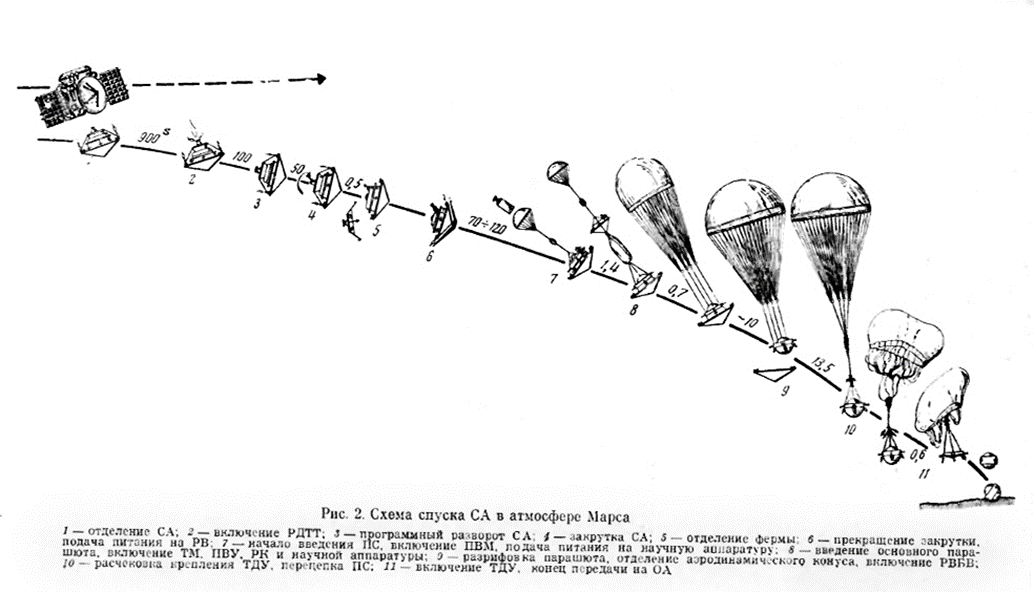
\includegraphics[width=.95\textwidth]{12uaYg.png}
\end{center}

\subsubsection*{Aufgabe 2.}
Der nächste Schritt besteht darin, den Hauptfallschirm zu aktivieren und zu
öffnen. Es ist dabei mehrere Operationen umzusetzen: Öffnen des
Fallschirmfachs, Entfernen des oberen Deckels, den Hauptfallschirm vollständig
zu öffnen und schließlich zu verhindern, dass der Hauptfallschirm die
Landekapsel am Boden überdeckt. Analysieren Sie das Bremssystem der
Landekapsel, identifizieren Sie alle unerwünschten Wirkungen, die beim Bremsen
auftreten können, formulieren Sie diese Widersprüche. Welche Konstruktionen
können an der Beseitigung dieser unerwünschten Wirkungen beteiligt werden?
\begin{center}
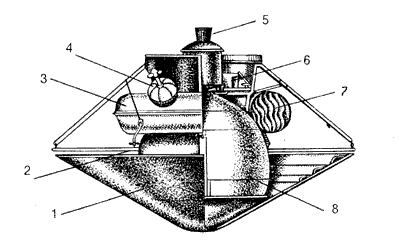
\includegraphics[width=.4\textwidth]{GIj0Ml.png}\hfill
  \begin{minipage}[b]{.55\textwidth}\small
    Landekapsel der Station Mars-2:
    \begin{itemize}[noitemsep]
    \item[1] -- aerodynamischer Kegel;
    \item[2] -- Antenne des Funkhöhenmessers;
    \item[3] -- Fallschirmcontainer;
    \item[4] -- Antrieb des Deckels des Auswurf-Fallschirms;
    \item[5] -- Antrieb zur Steuerung der Landekapsel;
    \item[6] -- Instrumente und Apparate des Steuerungssystems;
    \item[7] -- Hauptfallschirm;
    \item[8] -- automatische Marsstation
    \end{itemize}
  \end{minipage}
\end{center}
Diese Geschichte hat eine unerwartete und interessante Fortsetzung.

\subsubsection*{Aufgabe 3.}
Sie haben sich noch nie gefragt, was über gebrauchte Apparate bekannt ist, die
auf dem Mond, dem Mars oder der Venus zurückgeblieben sind?  Die Erforschung
der Resultate vernünftiger Aktivitäten auf den Planeten und ihren Satelliten
hat sich noch nicht zu einer eigenständigen Domäne entwickelt, aber
Publikationen zur „Weltraumarchäologie“ gibt esw schon recht viele.  Man
könnte denken, dass die Landeplätze aller Apparate, die Planeten und deren
Satelliten erkundet haben, genau bekannt, aber... Vitaly Yegorov beschreibt
diese Aufgabe so: „Als ich mir die Website von \emph{HiRise}\footnote{High
  Resolution Imaging Science Experiment} anschaute, fand ich nur ein Bild aus
dem Jahr 2007 mit dem Titel \emph{Center of Soviet Mars 3 Landing Ellipse}.
Das war für mich eine Entdeckung, weil ich mir der Allmacht von NASA und
HIRise so sicher war, dass ich erwartet hatte, eine genaue Angabe vorzufinden,
wo diese Station steht.  Eine kurze Suche im Internet ergab ebenfalls kein
Ergebnis. Es war also offensichtlich, dass Mars-3 nie gefunden worden war. Ich
lud das Foto im Vollformat (1.3 GB) herunter, öffnete es und verstand, warum
in fünf Jahren niemand die Station gefunden hat. (Das Bild hat eine Auflösung
von 30 cm pro Pixel, d.h. ein Objekt der Größe von 30 cm entspricht einem
Punkt.  Mars-3 ist ein 1.5\,m großes Objekt -- im Bild ein Objekt aus
$6\times6$ Pixeln). Stellen Sie sich eine Suche eines abgerundeten, 1.5 Meter
breites Objekts in einem Rechteck von $6\times20$ Kilometern vor.  Ich weiß,
viele Leute dachten sofort daran, dass man ein Programm schreiben muss, das
nach der Station sucht. Aber ich glaube nicht, dass eine Suche ohne KI möglich
ist. Ja, das Programm könnte interessante Felsblöcke von angemessener Größe
hervorheben.  Aber da gibt es Tausende solcher Objekte, denn in der Nähe
befindet sich ein Krater, aus dem fächerförmig Steine flogen.“

Was würden Sie in dieser Situation vorschlagen? Wie finden Sie Mars-3? Und die
Hauptsache ist, warum überhaupt die Ergebnisse intelligenter menschlicher
Aktivitäten auf Planeten und Satelliten erforschen, welche Informationen
können wir erhalten?

\subsubsection*{Aufgabe. Der gefährliche Planet.}
Eine fantastische Geschichte beschreibt einen erstaunlichen Planeten. Alles
darauf ist wie auf der Erde: die gleiche Atmosphäre, die gleichen Pflanzen und
Tiere. Aber die Insekten und Vögel fliegen mit Überschallgeschwindigkeit.
Lassen Sie uns nicht näher darauf eingehen, wie sie das tun.  Das ist nicht
der Punkt. Sie wissen wahrscheinlich, dass eine Flugzeugkollision mit Vögeln
zu Unfällen führt. Aber hier ist die Luft gefüllt mit lebendigen „Kugeln“ und
„Granaten“...  Es wurden zwei Astronauten auf dem Planetebn abgesetzt, und man
schaffte es gerade noch, sie zu retten. Sogar ein gepanzertes Geländefahrzeug
wurde schnell von Überschallfliegen zerstört...  Stellen Sie sich vor, Sie
wären auf der Expedition zu diesem Planeten. Machen Sie Vorschläge, wie Sie
und die Besatzung in Sicherheit zu bringen sind.

Stellen wir uns die umgekehrte Situation vor. Auf dem Planeten, den wir
untersuchen, wurde es intelligentes Leben entdeckt. Die Geschwindigkeit der
Veränderung, die Reaktionsgeschwindigkeit der intelligenten Wesen ist jedoch
im Vergleich zu Menschen viele Male verlangsamt. So langsam, dass ein Moment
für einen Menschen für die Wesen auf dem fremden Planeten Jahre
dauert\footnote{HGG: Eigentlich ist es umgekehrt -- ein Moment für die fremden
  Wesen dauert mehrere Menschenjahre.}. Wie stellt man Kontakt her, wie
verhandelt man?

\subsection{Nomination „Fantasieren“}

\subsubsection*{Aufgabe 1.}
Heutzutage gehen Astronauten in Raumanzügen ins All, die es ihnen erlauben, zu
atmen und die sie vor Strahlung schützen. Kann eine Person im Kosmos ohne
Raumanzug leben? Bisher nicht wirklich, noch nicht, aber
Fantasy-Schriftsteller haben darüber geschrieben, wie es klappen könnte.
Denken auch Sie sich etwas aus. Nutzen Sie dabei einen der Tricks der
TRIZ-Phantasietechnik.

\subsubsection*{Aufgabe 2.}
In Hal Clements Roman \emph{Unternehmen Schwerkraft} spielt sich die Handlung
auf einem Planeten ab, auf dem die Schwerkraft 800 Mal so groß ist wie auf der
Erde.  Denke dir einen fantastischen Planeten aus, der sich von der Erde durch
einen anderen Parameter unterscheidet. Beschreibe die Abenteuer einer
Raumschiffbesatzung auf einem Planeten wie diesem.

\subsection{Nomination „TRIZ-Werkzeuge“}

\subsubsection*{Aufgabe 1.}

\newcommand{\CosmicInventions}{Kosmische Reisen und Forschungen ist ein Traum
  vieler Generationen mutiger Menschen. Diese Forschungen haben auch rein
  praktische Anwendungen. Sie wissen sicher, dass die Teflon-Beschichtung,
  drahtlose Elektrowerkzeuge, Geolokalisierungsdienste und viele andere
  Erfindungen, die unser Leben komfortabler und sicherer machen, in der
  Kosmos-Industrie gemacht wurden. Die Aufgaben in der Nomination
  „TRIZ-Werkzeuge“ sind genau mit solche Erfindungen verbunden.
\begin{itemize}[noitemsep]
\item[1)] Stellen Sie einen Katalog von „Weltraum-Erfindungen“ zusammen, die
  Anwendungen im Alltag fanden.
\item[2)] Formulieren Sie die Widersprüche, die mit diesen Erfindungen gelöst
  wurden.
\item[3)] Schlagen Sie eine ungewöhnliche Verwendung dieser Erfindungen zur
  Lösung von noch nicht gestellten Aufgaben vor.
\end{itemize}}

\CosmicInventions

\subsection{Nomination „Forschung“}

\subsubsection*{Aufgabe 1.}

\AnimalsInCosmos

Ist es möglich, im Orbit ähnliche Bedingungen zu schaffen wie in komplexen
natürlichen Systemen wie z.B. einem Wald, einer Wiese, usw., wo Tiere und
Pflanzen miteinander interagieren?  Gibt es solche Projekte bereits,
welche Probleme haben sich bei  deren Realisierung ergeben?  

\subsubsection*{Aufgabe 2.}
In jeder Familie gibt es Geschichten, die von Generation zu Generation
weitergegeben werden: vom Großvater, der von Chicago nach Russland kam, von
seiner Großmutter, die Leben an der Front gerettet hat, usw. Es gibt tragische
Fälle, es gibt komische Fälle, aber man erinnert sich an sie wegen ihrer
Klarheit, sie werden gern viele Male wiedererzählt, werden vom Vater zum Sohn
weitergegeben. Um die wahren Geschichten wachsen legendäre Details.
Beschreiben Sie die Geschichte Ihrer Familie: seit wann und woher Ihre Familie
stammt, welche besonderen Taten Ihre Vorfahren vollbracht haben, welche
besonderen Geschichten haben Ihre Familie begleitet. Schreiben Sie das auf,
was Sie über Ihre Familie mitteilen möchten.  Wenn Sie die Geschichte über
Ihre Familie beendet haben, geben Sie einen Kommentar zu der Geschichte ab.
stellen Sie sich vor, Ihre Geschichte würde im 25. Jahrhundert gelesen, und
man weiß dort nichts anderes über unserer Zeit. Wie wird unsere Zivilisation
in deren Augen aussehen, wenn sie nur auf der Grundlage Ihrer
Familiengeschichte studiert würde? Was würden Sie in Ihrer Geschichte
verändern, damit sie von den Menschen auch nach vielen Jahrhunderten
verstanden wird?

\subsection{Nomination „TRIZ-Videos“}
\subsubsection*{Aufgabe 1.}\VideoOne
\subsubsection*{Aufgabe 2.}\VideoTwo

\GeneralText
\clearpage

\section{Kategorie 15-17 Jahre}

\subsection{Nomination „Erfinden“}

\newcommand{\Aberration}{Es ist bekannt, dass sich das gebrochene Sonnenlicht
  in ein Spektrum zerlegt. Die Astronomen haben sehr darunter gelitten. In den
  Linsen des Teleskops wird auch das Licht von Sonne, Planeten und Sternen
  gebrochen. Und kosmische Objekte sind von bunten Auren umgeben, was daran
  hindert, sie richtig zu beobachten. Dieses Phänomen wird als „chromatische
  Aberration“ bezeichnet. Der große englische Physiker I. Newton hielt es für
  unmöglich, sie loszuwerden.  Schlagen Sie eine Methode zur Herstellung von
  Linsen vor, die keine chromatische Aberration verursachen.}

\newcommand{\CosmicOperation}{Obwohl nur starke und gesunde Menschen als
  Kosmonauten akzeptiert werden, kann in den Raumstationen der nahen Zukunft
  viel mit ihnen passieren. Es ist möglich, dass eine komplizierte Operation
  erforderlich wird. Auf der Erde wird der Patient auf den Operationstisch
  gelegt, wo sowohl der Patient als auch der Tisch, die Instrumente und Ärzte
  durch die Schwerkraft in ihrer Position gehalten werden. Aber in der
  Schwerelosigkeit ist das nicht so einfach. Auf den ersten Blick kann ein
  Tisch an den Boden geschraubt werden. Aber Ärzten kann man nicht
  festschrauben. Sie müssen sich bewegen. Auch die Instrumente und die
  Behälter mit Präparaten kann man nicht verschrauben. Auch den Kranken kann
  man nicht immer festbinden -- er könnte dabei weitere Verletzungen erleiden.
  Und wenn die Operation schwerwiegend ist, eine umfassende Öffnung des
  Körpers erfordert, müssen auch die inneren Organe vom „Fliegen“ abgehalten
  werden.  Schlagen Sie einen Entwurf für den Operationssaal vor,
  Operationstisch, Werkzeuge und Vorrichtungen für die unterschiedlichsten
  Operationen in der Schwerelosigkeit.}

\subsubsection*{Aufgabe 1.}\Aberration
\subsubsection*{Aufgabe 2.}\CosmicOperation

\subsection{Nomination „Fantasieren“}
\end{document}
\subsubsection*{Aufgabe 1.}
В «этажной схеме» Г. Альтшуллера существует четыре способа («этажа»), с
помощью которого можно придумать новую фантастическую идею. Изучите эту схему.
Придумайте и опишите идеи третьего и четвертого этажей для объекта «скафандр».

\subsubsection*{Задание 2.}
В фантастическом романе Ларри Нивена «Интегральные деревья» люди живут на
планете, которая представляет собой огромное дерево, летающее в космосе по
орбите вокруг звезды, похожей на Солнце. В романе Пола Шеффилда «Мир – кольцо»
люди живут на поверхности огромного кольца, вращающегося вокруг звезды.
Придумайте и опишите фантастическую планету, используйте для этого
какой-нибудь прием фантазирования. Напишите небольшой рассказ о приключениях
на придуманной вами планете.

\subsection{Номинация «Инструменты ТРИЗ»}

\newcommand{\BlackBox}{С помощью морфологической таблицы (см. «краткий анализ
  задачи «О черном ящике цивилизации») сформулируйте исследовательскую тему,
  подзадачу для задачи о “черном ящике” цивилизации. Соберите примеры, задачи
  по выбранной вами теме. Проанализируйте собранную информацию. Какие способы
  передачи информации о современной цивилизации вы можете предложить? Что,
  по-вашему мнению, можно сделать сегодня для сохранения информации о нашей
  цивилизации?}

\subsubsection*{Задание 1.}\BlackBox
\subsubsection*{Задание 2.}\CosmicInventions

\subsection{Номинация «Исследования»}

\newcommand{\BlackBoxOfCivilization}{
\subsubsection*{Задача о “черном ящике” цивилизации.}
(цитируется по: Г.С. Альтшуллер, И.М. Верткин, “Как стать еретиком. Жизненная
стратегия творческой личности”, задачник; сборник “Как стать еретиком”,
Петрозаводск, “Карелия”, 1991 г., стр. 166-168).

“В крупных современных самолетах встроен так называемый “черный ящик”. Он
предназначен для записи режимов полета. В случае аварии легко выяснить ее
причины, установить виновных. Если авария произошла по вине летчиков или из-за
недостатков конструкции самолета, анализ записи позволяет будущие полеты
сделать безопаснее. Предотвратить происходящую аварию, помочь терпящим
бедствие “черный ящик” не способен, да это и не входит в его функции. Главная
его цель – работа на “завтра”; “черный ящик” позволяет учиться на чужих
ошибках.

В последнее время этими устройствами стали снабжать и океанские
лайнеры. Очевидно, в недалеком будущем “черные ящике” станут обязательными
атрибутами всех видов общественного транспорта, а, возможно, и личных
мото-транспортных средств.

Во все времена люди, отправлявшиеся в отчаянные путешествия, готовящиеся к
трагическим событиям, старались передать потомкам свой опыт, свое описание
происходящего. Обычно такие записи велись в трагических периоды людей: в
осажденных городах, в тюремных застенках, в ожидании близкой смерти. Вспомните
кумранские рукописи, дневник полярной экспедиции Скотта, записи самонаблюдений
Алена Бомбара.

Как правило, подобные “завещания” начинают составлять в последний момент,
когда остро ощущается нехватка времени и подходящих условий. Поэтому мы
знакомы лишь с единичными записями, чудом дошедшими до нас. Ко всему, - в том
числе (а может быть, в первую очередь) и к катастрофам, - надо готовиться
заранее.

Наша Земля не менее уязвима, чем любой другой “общественный вид транспорта”. В
прежние времена причиной будущего “конца света” считались некие мистические
силы “свыше”. В недалеком прошлом эту роль передали таинственным космическим
пришельцам, враждебно настроенным к землянам. Сейчас говорят, что главный наш
враг – мы сами, и предрекают генетический, социальный, демографический,
ядерный, экологический и прочие подобного рода кризисы. В общем-то, неважно, в
результате чего может произойти катастрофа, по этим или по еще неведомым
причинам; главное, что это в принципе возможно. Значит, Земле необходим свой
“черный ящик”. Он должен зафиксировать истинные причины возможной трагедии,
сохранить запись в целости нужное время и передать ее будущим поколениям:
опыт, особенно столь отрицательный и глобальный, бесценен.

Только будущее может однозначно ответить на вопрос о сегодняшней актуальности
“черного ящика” для планеты. Одно можно сказать уверенно уже сейчас: эта
проблема не надумана. Если она не “горящая”, - прекрасно, значит, у нас есть
время спокойно, тщательно подготовиться к ее решению. Если времени в обрез, -
что ж, надо успеть сделать то, что еще можно успеть. Словом, чем раньше
начнется разработка этой проблемы, тем лучше.

Решение проблемы во многом зависит от масштабов вероятной катастрофы. Возможно
несколько вариантов:
\begin{itemize}[noitemsep]
\item[а)] В результате катастрофы исчезнет половина населения Земли. Связь
  между городами сохранится. В какой-то степени сохранится прежняя
  инфраструктура.
\item[б)] На Земле останется несколько десятков тысяч человек. Связи
  практически не будет никакой. Остатки населения довольно быстро деградирует,
  к примитивным ремеслам, к примитивной технике. Пройдет много времени, прежде
  чем вновь возникнут условия для ощутимого рывка вперед.
\item[в)] Разумная жизнь вовсе исчезнет с лица Земли. Лет через 100-150
  возникнут условия, приемлемые для жизни человека, но, когда произойдет
  возрождение Разума – “одному аллаху ведомо”.
\item[г)] С Земли исчезнет всякая жизнь. Время восстановления условий –
  миллиард лет.
\end{itemize}
Давайте остановимся на самом трудном – последнем варианте. Если удастся
придумать что-то для преодоления обостренного конфликта, в более мягких
условиях задача тем более будет решена.

Итак, условия проблемы. Через 100-150 лет произойдет исчезновение всякой жизни
с Земли. Возможное время восстановления - миллиард лет. Как передать “черный
ящик” на такую временную дистанцию? Что в него записать?

Это очень сложные вопросы. Например, вопрос о технике передачи
информации. Ведь сегодня неизвестно – кому придется передать информацию: кто
знает, какой вид примет разумная жизнь через миллиард лет после нашей эры… Да
и возникнет ли она самостоятельно на Земле? Как помочь в восстановлении
разумной жизни? Как сохранить генофонд нашей флоры и фауны? Как сделать так,
чтобы информация попала вовремя: когда уже были бы способны понять, о чем идет
речь, и еще было бы не поздно? Как сделать так, чтобы информацию смогли без
труда расшифровать? Как сохранить запись на такой временной дистанции? Как
сделать так, чтобы информации поверили, чтобы не восприняли ее как глупую
шутку соотечественников?

Не менее не ясен пока и вопрос о содержании “черного ящика”. Скорее всего,
“ящик” должен состоять из двух частей: “оперативной” (о причинах аварии) и
“стационарной” (о накопленной культуре, знаниях на Земле). Как постоянно
пополнять “оперативную” часть, включая непосредственно момент и последующее
время? Что записать в “стационарную” часть? “Все знания мира”? Что конкретно?
Каковы критерии отбора? Какие рекомендации мы можем передать будущей разумной
жизни для предотвращения аналогичных трагедий?

Вопросов много…

Чем хороша проблема? “Передача информации” на сегодня – тема для
первооткрывателя, абсолютно свободная от конкуренции, по крайней мере, на
ближайшие 30-50 лет (надеемся, что разум все-таки возобладает и человечество
осознает проблему раньше случившейся катастрофы). Это одна из немногочисленных
тем, полностью лишенных отрицательной стороны. Тема максимально
благородная. Предельно общественно-полезная. Супермасштабная – совершенно
очевидно уже сейчас, что эта тема на всю жизнь, причем не на одну. Тема имеет
социальный и технический аспекты, т.е. подходит для человека с любой
специализацией.

(Заранее можно предсказать типовое ханжеское возражение против этой проблемы:
когда горит дом, надо не записывать, отчего произошел пожар, а таскать ведра с
водой. Возможная катастрофа цивилизации ставит много проблем, большинство из
которых воспринимается пока весьма абстрактно. Основная часть населения
планеты продолжает работать на предприятиях своих государств, т.е. продолжает
участвовать в уничтожении природы. Немногие бьют в колокола и пытаются тушить
разгорающееся пламя. Но никто, ни один человек на всей Земле даже близко не
подошел к проблеме “черного ящика”! Как знать, возможно, письмо, отправленное
на миллиард лет вперед, важнее двух сегодняшних ведер воды…)”.}

\BlackBoxOfCivilization

\subsection{Номинация «Видеоролики по ТРИЗ»}

\newcommand{\VideoThree}{Проиллюстрируйте с помощью средств кино или анимации
  решение изобретательских задач. Это могут быть как технические решения, так
  и изобретения в нетехнических областях. }

\subsubsection*{Задание 1.}\VideoOne
\subsubsection*{Задание 2.}\VideoThree

\GeneralText
\clearpage

\section{Категория студенты}

\subsection{Номинация «Изобретательство»}

\subsubsection*{Задача 1.}\Aberration
\subsubsection*{Задача 2.}\CosmicOperation

\subsection{Номинация «Фантазирование»}

\subsubsection*{Задание 1.}
В цикле романов Грега Игана «Ортогональная вселенная» действие происходит во
вселенной, где скорость света зависит от длины волны. Придумайте и опишите
вселенную, в которой изменен какой-нибудь другой физический закон или мировая
постоянная.

\subsubsection*{Задание 2.} 
В цикле романов Стивена Бакстера и Терри Пратчетта «Бесконечная Земля» описаны
миры, в каждом из которых существует Земля, отличающаяся от нашей планеты тем,
что на каком-то этапе эволюция пошла иначе, чем в нашей реальности. В одном
случае динозавры не погибли, в другом вся планета оказалась покрытой лесами, в
третьей нет людей, но есть разумные собаки…  Придумайте космический фактор,
который когда-то изменил ход эволюции на Земле, и опишите, какой в результате
действия этого фактора стала планета в наши дни.

\subsection{Номинация «Инструменты ТРИЗ»}

\subsubsection*{Задание 1.}\BlackBox
\subsubsection*{Задание 2.}\CosmicInventions

\subsection{Номинация «Исследования»}

\BlackBoxOfCivilization

\subsection{Номинация «Видеоролики по ТРИЗ»}

\subsubsection*{Задание 1.}\VideoOne
\subsubsection*{Задание 2.}\VideoThree

\GeneralText
\clearpage

\section{Краткий анализ задачи о “черном ящике” цивилизации. }
\begin{center}
  © Рубин М.С.
\end{center}
Задача о “черном ящике” цивилизации была предложена как генератор новых
исследовательских тем, источник Достойной Цели для исследователей.  

“Г.С. Альтшуллер и И.М. Верткин выделяют три яруса тем:
\begin{itemize}[noitemsep]
\item темы узкотехнические, узко-научные, узко-художественные, например,
  изобретение ракет;
\item темы общетехнические, общенаучные, общехудожественные, например,
  развитие космонавтики;
\item темы, затрагивающие цивилизацию в целом (социально-технические,
  социально-научные, социально-художественные и пр.), например, проектирование
  космической цивилизации или цивилизации с телевидением.
\end{itemize}
С исследовательской точки зрения эффективнее всего работать с темами третьего
яруса - на уровне общечеловеческих проблем. Здесь самый большой простор для
развития тем, наименьшая вероятность "застрять" на мелкотемье или оказаться в
ситуации острой конкуренции с другими исследованиями. В качестве примера мне
хотелось представить хотя бы одну проблему общечеловеческого уровня. Речь
пойдет о проблеме создания "черного ящика" на случай всемирной катастрофы.
("Как стать еретиком", Карелия, 1991, стр. 166-168).

Очень не многие из специалистов по ТРИЗ работали над предложенной задачей, еще
меньше публикаций на эту тему. Задача сложная и мы решили предложить некоторые
подходы к ней. Это лишь наш взгляд, и мы не претендуем на то, что это
единственный подход к задаче о “черном ящике” цивилизации.

Нам сразу хотелось бы отсечь очевидно слабые решения. Например: создание
глобальных систем сбора информации от каждого жителя Земли и размещение ее на
каком-нибудь спутнике Земли или Венеры. Не смотря, на очевидность
невыполнимости, не идеальности, подобные идеи все равно
высказываются. Исследовательская тема будет тогда интересной и сильной, когда
она будет направлена на разрешение противоречий, заложенных в задаче о “черном
ящике” цивилизации (например, информации должно быть очень много, чтобы
отразить все стороны цивилизации, и должно быть мало, чтобы ее легче было
сохранить и донести до потомков; или место хранения информации должно быть
близко, чтобы легче было размещать информацию, и должно быть далеко, чтобы
информация надежнее сохранялась при катастрофе), и максимально приближаться к
идеальному конечному результату (например, катастрофическая сила, разрушающая
цивилизацию САМА сохраняет ее для потомков).

Во время конференции школьников и студентов по ТРИЗ “ИКАРиада-2001” была
предложена морфологическая таблица для анализа задачи:

\begin{center}\small
  \begin{tabular}{|*{6}{>{\raggedright}p{1.9cm}|}c|}\hline
1. Какой объект & 1.1 Семья & 1.2. Дом & 1.3. Город & 1.4 Страна & 1.5. Весь
мир & \ldots \\\hline
2. Кому, куда & 2.1. Другим людям & 2.2. Другому государству & 2.3. Потомкам
через 50 (100, 1000) лет & 2.4. Иноземным цивилизациям & 2.5. Необитаемой
планете & \ldots \\\hline
3. Цель & 3.1. Сохранить информацию & 3.2. Избежать ошибок & 3.3. Сохранить
цивилизацию & 3.4. Возродить цивилизацию & 3.5. Расширить границы цивилизации
& \ldots \\\hline
4. Ресурсы & 4.1. Ресурсы сохраняемой системы & 4.2. Ресурсы уничтожающей силы
& 4.3. Ресурсы современной внешней среды & 4.4. Ресурсы среды, в которую
попадает “Черный ящик” & \ldots & \\\hline 
5. Причина катастрофы & 5.1 Естественные & 5.2. Социальные конфликты &
5.3. Природные катаклизмы & 5.4 Межличностные конфликты & 5.5. Террор и
преступления & \ldots \\\hline
  \end{tabular}
\end{center}
Эта таблица может быть использована для формулировки множества подзадач,
например, вариант (1.3-2.3-3.2-4.1-5.1) может быть сформулирован следующим
образом: как сохранить информацию о современном Петрозаводске для поколения
людей 22-го века в целях избегания повторения допущенных ошибок силами самого
города, если он будет изменяться в результате естественной эволюции. Уровень
формулированных задач и их остроту можно изменять по собственному вкусу.

Имеется очень широкий выбор направлений ведения дальнейших исследовательских
работ по теме “черного ящика цивилизации”. Можно, например, уточнить оси
морфологического ящика: их количество и содержание. Можно сделать подборку
конкретных задач, собранных в рамках общей темы “черного ящика
цивилизации”. Можно провести анализ каждой из подзадач: сформулировать
противоречия, ИКР, проанализировать ресурсы. Можно выстроить иерархию задач
темы “черного ящика цивилизации”. Можно собрать информацию о наиболее частых
причинах гибели цивилизаций. Очень плодотворным может стать анализ методов
восстановления информации, которые имеются в археологии и у
историков. Возможностей для ведения исследовательской работы, действительно
очень много.

Очень эффективным можно считать сбор различных картотек (см. статью М. Рубина
“Личные картотеки – фундамент творчества”, статья опубликована на сайте
ОТСМ-ТРИЗ-технологий  \url{http://www.triz.minsk.by/e/221001.htm} ) по теме
“черного ящика цивилизации”.

Можно, например, начать с картотеки "черных ящиков" - с самолетов разного
типа, океанских лайнеров или других систем. Любопытно выяснить характер
фиксируемой информации, основные проблемы и противоречия "черных ящиков",
сделать прогноз их развития. Может оказаться, например, что "Черный ящик
цивилизации" - логическое продолжение развития обычных "черных
ящиков". Попутно можно предложить новые идеи и решения в этой области.

Очень важный вопрос: что именно передавать потомкам или пришельцам о погибшей
цивилизации. Для ответа на него может оказаться другая картотека - о КЛЮЧЕВЫХ
НАХОДКАХ (памятников), помощью которых удалось раскрыть тайны погибших
цивилизаций.
\medskip

Приведу только один пример. Для изучения погибшей цивилизации майя очень важно было расшифровать письменность этого народа. Сделать это удалось, главным образом, с помощью двух документов:
\begin{itemize}
\item рукописи "Сообщение о делах в Юкатане" времен завоевания испанцами
  индейцев майя, где, в частности, приводился сокращенный алфавит майя с его
  "ОЗВУЧИВАНИЕМ" ИСПАНСКИМИ буквами;
\item записям древних мифов (книги Чилам Балам), сделанных в XVI веке
  ЛАТИНСКИМИ БУКВАМИ и отражающих язык майя времен начала нашей эры.
\end{itemize}
К этому, безусловно, необходимо добавить дошедшие до нас современные (живые)
языки майя и испанцев, а также сведения об испанском языке ХYI века.

Любопытно отметить, что "черные ящик" цивилизации майя дошел до нас в виде
бисистемы: в первую очередь это сами города древних майя с храмами, надписями
на них, картинками, рисунками, а также ключ к их объяснению - алфавит, о
котором мы только что упоминали.
\medskip

При самом трудном варианте (с Земли исчезает всякая жизнь) живой язык,
естественно, не сохранится. Так, например, произошло с шумерскими текстами: их
удалось полностью расшифровать, но никто не знает, как звучал этот
язык. Необходимо совмещение предмета или действия (показанных в различных
ситуациях) с его письменным и звуковым (речевым) изображением. Что-то вроде
телевизионных комиксов для изучения иностранных языков.

Пример "черного ящика" цивилизации древних майя наводит на интересную
мысль. Дело в том, что рукопись "Сообщение о делах в Юкатане" - основной,
наиболее полный и точный документ о древней цивилизации - была составлена
епископом-испанцем Диего де Ланда. Именно под его руководством тщательнейшим
образом было уничтожено почти все письменно и другое культурное наследие майя
(за эту свою деятельность де Ланда и получил звание епископа). Рукопись де
Ланды - своеобразный отчет перед начальством о проделанной "работе" по
истреблению ереси. Возникает любопытная гипотеза: причина, приводящая к
катастрофе (например, испанцы в лице Диего де Ланды) САМА создает "черный
ящик" (знаменитую рукопись епископа). Второй документ-ключ к разгадке текстов
майя - "Книги Чилам Балам", написанные на латинице - имеют примерно такой же
характер происхождения, как и рукопись де Ланды. Испанцы запрещали майя
пользоваться родной письменностью, и те стали записывать древние тексты на
дозволенной латинице. Все та же ситуация: испанцы, своими запретами, САМИ
вынудили майя создать документ о своей культуре, понятный для потомков. Еще
один пример, о котором мы уже вспоминали: извержение Везувия уничтожило
Помпеи, но оно же и сохранило для нас этот город, засыпав его толстым слоем
пепла.
\medskip

Итак, сила, приводящая к катастрофе, САМА создает "черный ящик" в момент
катастрофы. Что это - гипотеза, идеальный вариант решения проблемы или
закономерность образования "черных ящиков" цивилизаций? Ответить на этот
вопрос поможет картотека КЛЮЧЕВЫХ НАХОДОК к разгадке культуры погибших
цивилизаций: с помощью чего удалось расшифровать информацию о жизни людей. В
связи с этим можно вспомнить и о многочисленных примерах ключевых находок
древних животных: мамонтов, неандертальцев, динозавров.

Общеизвестна, например, находка очень хорошо сохранившегося динозавра из рода
аллозавров. Эта находка стала настолько важной для науки, что останки этого
динозавра назвали по имени – Большой Ал. Хорошо сохранился не только скелет,
но отпечаток сердца. Ученым удалось восстановить с абсолютной точностью
особенности поведения аллозавров, среду их обитания, скорость передвижения,
повадки. Удалось даже сделать жизнеописание Большого Ала: в каком возрасте,
какие травмы он получил, в каких ситуациях эти травмы и болезни могли
возникнуть, от чего умер этот динозавр, живший 45 миллионов лет назад. Уже
старый и больной Большой Ал отправился к реке во время засушливого
лета. Дождей не было, и вода все не приходила. Обессиленный, он ждал воду в
русле высохшей реки. Вскоре вода пришла, но Большой Ал уже умер. Ил обволок
тело и сохранил его для нас на многие миллионы лет. Река, убившая динозавра,
САМА же сохранила информацию о нем.
\medskip

Возможно, что с помощью одной только разрушающей цивилизацию силы не удастся
найти абсолютно надежный механизм создания в нужный момент "черного
ящика". Тогда возникает новая задача: как сделать, чтобы "черный ящик" был
полезен и необходим при нормальном течении жизни без катастроф. Это позволило
бы сделать весь проект создания "черного ящика" цивилизации гораздо дешевле,
повысило бы вероятность его реализации, обеспечило бы надежность его
функционирования в до катастрофический период.

Как и всякая сверхпроблема, проект "Черный ящик" дает целый спектр задач,
проблем и тем для исследования. Представлю еще одну из них, но прежде -
карточка из моей картотеки:

"Кто спасется в катастрофе".

"С момента вступления в ядерную эпоху перед сверхдержавами постоянно стоит
дилемма - чье выживание обеспечить в первую очередь в случае крупномасштабного
конфликта: населения страны или высших эшелонов власти? В самом начале своего
восьмилетнего пребывания у власти президент Рейган, отбросив предрассудки
"холодной войны" с ее ориентацией на гражданскую оборону, заявил, что в
ядерной войне можно победить, но лишь в том случае, если будет обеспечено
выживание высших гражданских и  военных руководителей. Процедура эвакуации
предусмотрена для представителей высших эшелонов власти, выживание которых
считается необходимым для "обеспечения непрерывности государственной власти" -
всего для более 1000 человек".  ("Комсомольская правда", 26.08.1989).

Аналогичные программы имеются не только в США, но и в других странах. В
результате реализации подобных проектов вполне возможна ситуация, при которой
после катастрофы на Земле останутся только "высшие эшелоны власти". Те ли это
люди, которые должны остаться и продолжить разумную жизнь на Земле? Они умеют
руководить государствами, которых не будет. Смогут ли эти люди выжить сами,
без своих подчиненных? Если современная цивилизация способна обеспечить
выживание только очень небольшой части человечества, то какие люди должны при
этом выжить? Какой социальный механизм должен обеспечить этот отбор? Чем
должны быть заняты люди во время вынужденной "отсидки", пока не восстановились
приемлемые условия на Земле? Удастся ли ответить на все эти вопросы без
решения задачи о “черном ящике цивилизации”.


\end{document}
